% -------------------------------------------------------------
% question_2.tex - Arknights Lone Trail pure TikZ vector asset
% Target: Replace 素材库/正文/question_2.png (526 x 285 bp)
% Supports dynamic colors: mibai, qiancheng, lv, huang, hong
% -------------------------------------------------------------
\ifcsname\string\color@mibai\endcsname\else\definecolor{mibai}{RGB}{244, 237, 218}\fi
\ifcsname\string\color@qiancheng\endcsname\else\definecolor{qiancheng}{RGB}{227, 101, 53}\fi
\ifcsname\string\color@lv\endcsname\else\definecolor{lv}{RGB}{131, 187, 170}\fi
\ifcsname\string\color@huang\endcsname\else\definecolor{huang}{RGB}{227, 164, 60}\fi
\ifcsname\string\color@hong\endcsname\else\definecolor{hong}{RGB}{149, 44, 38}\fi

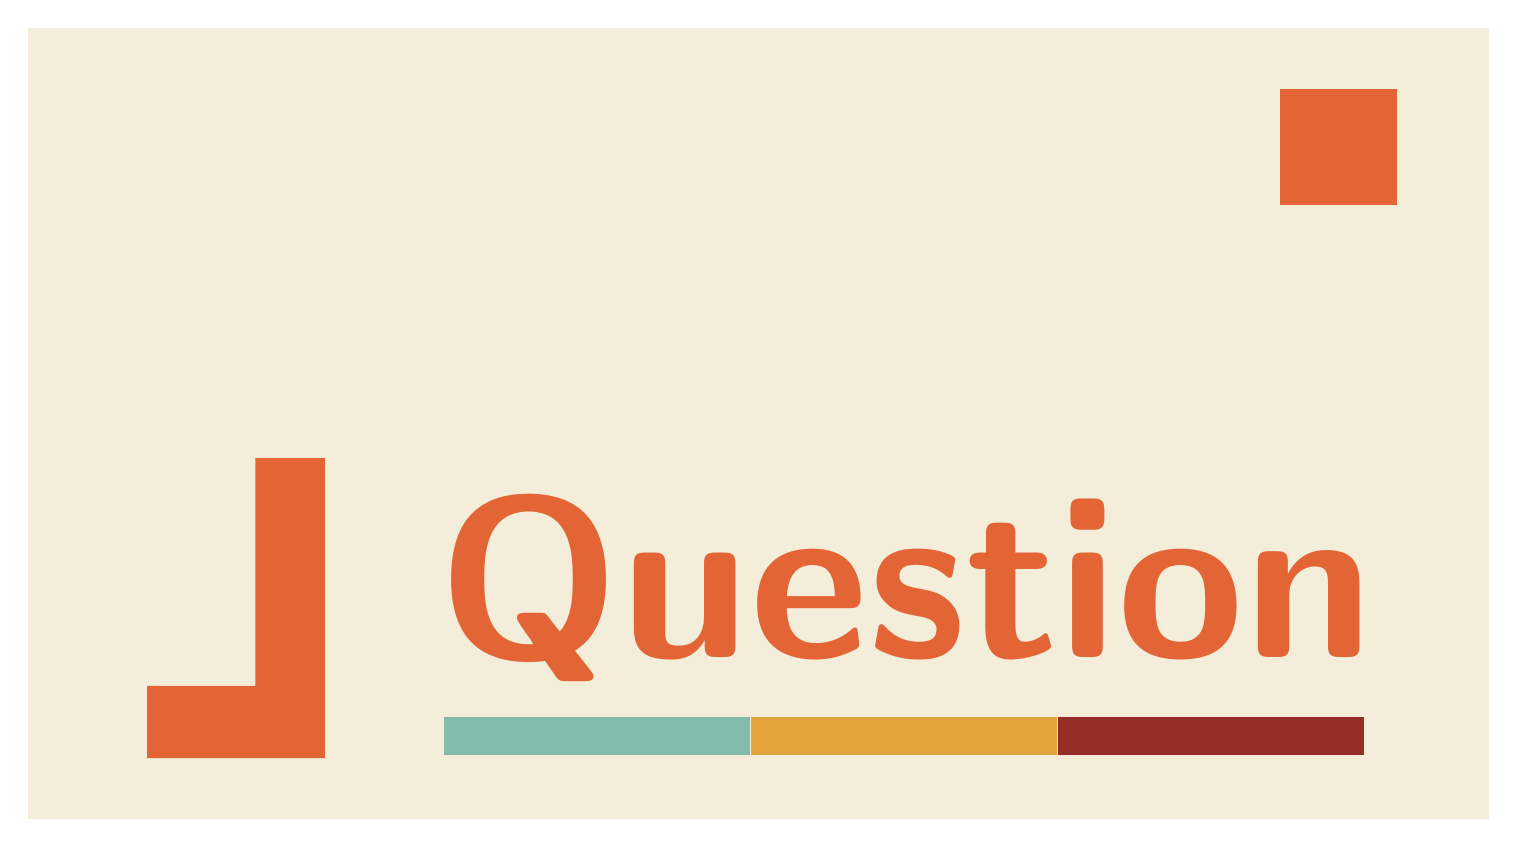
\begin{tikzpicture}[x=1bp, y=1bp, inner sep=0pt, outer sep=0pt]%
  % Bounding box & Background (exact 526 x 285 bp)
  \fill[mibai] (0, 0) rectangle (526, 285);

  % Upper-right orange square (42 x 42 bp, top margin 22 bp, right margin 33 bp)
  \fill[qiancheng] (451, 221) rectangle (493, 263);

  % Lower-left orange folded hook (base: 64 x 26 bp, stem: 25 x 82 bp)
  \fill[qiancheng] (43, 22) -- (107, 22) -- (107, 130) -- (82, 130) -- (82, 48) -- (43, 48) -- cycle;

  % Underline bars (height: 14 bp, Y: 23 to 37 bp)
  % Green bar (lv)
  \fill[lv] (150, 23) rectangle (260, 37);
  % Yellow bar (huang)
  \fill[huang] (260.5, 23) rectangle (370.5, 37);
  % Red bar (hong)
  \fill[hong] (371, 23) rectangle (481, 37);

  % Center text: Bold sans-serif "Question" (color: qiancheng)
  \node[anchor=south west, text=qiancheng, inner sep=0pt] at (147.5, 49.5) {%
    \resizebox{337bp}{57bp}{%
      \ifdefined\AvantGarde\AvantGarde\else\sffamily\bfseries\fi Question%
    }%
  };
\end{tikzpicture}%
